\documentclass[12pt,a4paper]{article}
\usepackage[utf8]{inputenc}
\usepackage[spanish,es-tabla,es-noquoting]{babel}
\usepackage{geometry}
\usepackage{graphicx}
\usepackage{multirow}
\usepackage{tabularx}
\usepackage{longtable}
\usepackage{float}
\usepackage{amsmath}
\usepackage{amssymb}
\usepackage{mathptmx}
\usepackage{fancyhdr}
\usepackage{array}
\usepackage[table]{xcolor}
\usepackage{titlesec}
\usepackage{setspace}
\usepackage{microtype}
\usepackage{lastpage}
\usepackage{booktabs}
\usepackage{enumitem}
\usepackage{hyperref}
\usepackage{listings}

\hypersetup{
    colorlinks=true,
    linkcolor=black,
    citecolor=blue!70!black,
    urlcolor=blue!70!black
}

\graphicspath{{images/}{../images/}{./}}

\geometry{
    top=4.7cm,
    bottom=2.5cm,
    left=2.5cm,
    right=2.5cm,
    headheight=3.9cm,
    headsep=0.4cm
}

\setstretch{1.15}
\setlength{\parindent}{0pt}
\setlength{\parskip}{0.45em}
\setlength{\tabcolsep}{4pt}

\titleformat{\section}
  {\normalfont\fontsize{12}{14.5}\bfseries}{\thesection.}{0.6em}{\uppercase}
\titlespacing*{\section}
  {0pt}{1.8ex plus 0.4ex minus 0.2ex}{0.6ex plus 0.2ex}

\titleformat{\subsection}
  {\normalfont\fontsize{11.5}{13.5}\bfseries}{\thesubsection.}{0.5em}{}
\titlespacing*{\subsection}
  {0pt}{1.4ex plus 0.3ex minus 0.1ex}{0.4ex plus 0.1ex}

\titleformat{\subsubsection}
  {\normalfont\fontsize{10.5}{12.5}\bfseries\itshape}{\thesubsubsection.}{0.4em}{}
\titlespacing*{\subsubsection}
  {0pt}{1.1ex plus 0.2ex minus 0.1ex}{0.3ex plus 0.1ex}

\newcolumntype{Y}{>{\centering\arraybackslash}X}
\newcolumntype{L}{>{\raggedright\arraybackslash}X}
\newcolumntype{C}{>{\centering\arraybackslash}X}

\definecolor{headerred}{RGB}{180, 0, 0}
\definecolor{darkred}{RGB}{140, 0, 0}
\definecolor{lightgraybg}{RGB}{248, 248, 248}
\definecolor{tableheader}{RGB}{232, 238, 246}
\definecolor{navyheader}{RGB}{0, 52, 94}

\newcommand{\docCodigo}{TI-SIGE-ENT-F3-011}
\newcommand{\docVersion}{1.0}
\newcommand{\docProceso}{INGENIERÍA DE SOFTWARE / WORKFLOW DE APROBACIÓN}
\newcommand{\docElaboracion}{02/10/2026}
\newcommand{\docRevision}{02/10/2026}
\newcommand{\docTitulo}{MÓDULO DE REVISIÓN POR COMITÉ, OBSERVACIONES Y TRAZABILIDAD}
\newcommand{\docOrganizacion}{FACULTAD DE INGENIERÍA EN SISTEMAS, ELECTRÓNICA E INDUSTRIAL}
\newcommand{\docSubOrganizacion}{CARRERA DE INGENIERÍA DE SOFTWARE}

\newcommand{\encabezadofrecuente}{%
    \renewcommand{\arraystretch}{1.15}%
    \noindent\makebox[\textwidth][c]{%
    \begin{tabularx}{\textwidth}{|>{\centering\arraybackslash}m{2.8cm}|Y|>{\centering\arraybackslash}m{4.8cm}|}
        \hline
        \multirow{4}{2.8cm}{\centering\raisebox{-1.15cm}{
\includegraphics[width=2.5cm,height=2.0cm,keepaspectratio]{images/logo.png}}}
        & \textbf{\fontsize{9}{11}\selectfont \docOrganizacion} 
        & \textbf{\fontsize{8}{10}\selectfont CÓDIGO:} \fontsize{8}{10}\selectfont \docCodigo \\
        \cline{3-3}
        & \textbf{\fontsize{8.5}{10.5}\selectfont \docSubOrganizacion} 
        & \textbf{\fontsize{8}{10}\selectfont VERSIÓN:} \fontsize{8}{10}\selectfont \docVersion \\
        \cline{2-3}
        & \textbf{\fontsize{8}{10}\selectfont PROCESO:} \fontsize{8}{10}\selectfont \docProceso 
        & \textbf{\fontsize{8}{10}\selectfont ELABORACIÓN:} \fontsize{8}{10}\selectfont \docElaboracion \\
        \cline{2-3}
        & \textbf{\fontsize{8.5}{10.5}\selectfont \docTitulo} 
        & \textbf{\fontsize{8}{10}\selectfont ÚLTIMA REVISIÓN:} \fontsize{8}{10}\selectfont \docRevision \\
        \hline
    \end{tabularx}%
    }%
}

\pagestyle{fancy}
\fancyhf{}
\fancyhead[C]{\encabezadofrecuente}
\fancyfoot[C]{\fontsize{10}{12}\selectfont Página \thepage\ de \pageref{LastPage}}
\renewcommand{\headrulewidth}{0pt}

\lstset{
  basicstyle=\ttfamily\scriptsize,
  backgroundcolor=\color{lightgraybg},
  frame=single,
  breaklines=true,
  tabsize=2,
  showstringspaces=false
}

\begin{document}

\noindent{\fontsize{10.5}{12.5}\selectfont \textbf{Integrantes:} Heidi Villavicencio \quad$\vert$\quad Steeven Toala \quad$\vert$\quad Nixon Hurtado \quad$\vert$\quad Andrea Vásquez}

\vspace{0.25cm}

\section{Título}
\textbf{Denominación del Entregable:} Módulo de Revisión por Comité Académico, Historial de Observaciones y Circuito de Dictámenes -- Código EDT: 3.11 (Fase 3: Desarrollo Iterativo Core).

\section{Introducción}
El proceso de revisión académica en la FISEI UTA requiere un mecanismo transparente y auditable mediante el cual los Coordinadores de Área de Conocimiento, Coordinadores de Carrera y Comités de Calidad evalúen el contenido de los Planes de Trabajo e Informes Semestrales. En el esquema manual tradicional, las devoluciones se efectuaban mediante comentarios manuscritos o correos electrónicos informales, provocando pérdida de trazabilidad sobre qué aspectos fueron observados, quién los formuló y en qué versión del documento fueron subsanados.

Para resolver esta debilidad, se desarrolló el Módulo de Revisión por Comité en la solución SIGE. Este módulo implementa un motor de auditoría y dictámenes que soporta la máquina de estados documental, categorización de observaciones (menores, mayores y de forma), bloqueo transaccional de reenvíos no justificados y notificación al docente elaborador.

\section{Objetivo}

\subsection{Objetivo General}
Implementar y verificar el módulo de revisión por comités y coordinaciones académicas en la plataforma SIGE, proveyendo un circuito formal de dictámenes, registro histórico inmutable de observaciones y control de estados documentales.

\subsection{Objetivos Específicos}
\begin{itemize}[leftmargin=1.5em, itemsep=1.5pt]
    \item Implementar el modelo relacional de observaciones vinculadas por sección y por actividad en la base de datos PostgreSQL.
    \item Diseñar la interfaz de usuario en React para que los revisores emitan dictámenes (Aprobado, Observado, Rechazado) con comentarios enriquecidos.
    \item Garantizar la inmutabilidad del historial de observaciones para fines de auditoría del Sistema de Gestión de Calidad (SGC).
\end{itemize}

\section{Alcance}

\subsection{Límites de Implementación (In-Scope)}
\begin{itemize}[leftmargin=1.5em, itemsep=1.5pt]
    \item Panel de revisión para roles: Coordinador de Área, Coordinador de Carrera y Comisión de Calidad.
    \item Registro de observaciones a nivel global del expediente y a nivel específico por fila de la matriz de actividades.
    \item Notificación de estado al docente mediante eventos en base de datos y cambio visual de estado en el Dashboard.
\end{itemize}

\subsection{Exclusiones (Out-of-Scope)}
\begin{itemize}[leftmargin=1.5em, itemsep=1.5pt]
    \item Calificación cuantitativa con notas numéricas al desempeño del docente (la evaluación es cualitativa SGC: Conforme / No Conforme).
    \item Reasignación externa de revisores fuera de la estructura organizativa de la FISEI.
\end{itemize}

\section{Definiciones}
\begin{itemize}[leftmargin=1.5em, itemsep=2pt]
    \item \textbf{Dictamen Académico:} Resolución formal emitida por un miembro evaluador (Aprobado Conforme, Con Observaciones, Devuelto para Corrección).
    \item \textbf{Observación Subsanable:} Señalamiento de inconsistencia en fechas, horas o evidencias que el docente puede corregir sin rehacer el expediente completo.
    \item \textbf{Máquina de Estados Documental:} Ciclo de vida regulado en base de datos: \texttt{BORRADOR} $\rightarrow$ \texttt{ENVIADO\_REVISION} $\rightarrow$ \texttt{OBSERVADO} $\rightarrow$ \texttt{SUBSANADO} $\rightarrow$ \texttt{APROBADO}.
    \item \textbf{Trazabilidad SGC:} Capacidad de reconstruir la cronología completa de un documento, incluyendo autor, revisores, comentarios y marcas temporales de cada cambio.
\end{itemize}

\section{Responsabilidades}
\begin{itemize}[leftmargin=1.5em, itemsep=2pt]
    \item \textbf{Analista de Requisitos / UI-UX (Heidi Villavicencio):} Relevamiento y modelado de necesidades, especificaciones funcionales, diseño de interfaces de usuario y verificación de usabilidad.
    \item \textbf{Líder de Proyecto / Arquitecto de Software (Steeven Toala):} Arquitectura de software, gobierno técnico, cumplimiento metodológico del cronograma y control de calidad integral.
    \item \textbf{Desarrollador Backend / DBA (Nixon Hurtado):} Modelo de base de datos PostgreSQL, persistencia de datos, seguridad por roles y reglas lógicas de validación.
    \item \textbf{Desarrolladora Frontend / QA (Andrea Vásquez):} Implementación de componentes React, manejo de estado global, integración de APIs y ejecución de pruebas de aceptación.
    \item \textbf{Docente Evaluador / Tutor (Ing. Paulo Torres, Mg.):} Dirección académica, asesoría metodológica, revisión de suficiencia técnica y validación institucional de los entregables.
\end{itemize}

\section{Normativa Legal y Técnica}
\begin{itemize}[leftmargin=1.5em, itemsep=2pt]
    \item \textbf{ISO/IEC 25010 (Calidad de Software):} Requisitos de integridad, auditabilidad y confiabilidad de transacciones documentales.
    \item \textbf{ISO 9001:2015 (Cláusula 7.5):} Control y preservación de la información documentada del Sistema de Gestión de Calidad.
    \item \textbf{Reglamento de Régimen Académico Institucional UTA:} Procedimiento para la aprobación de la planificación y rendición docente ante comisiones académicas.
\end{itemize}

\section{Método, Políticas y Contenidos}
El flujo de revisión implementa políticas de seguridad y concurrencia optimista:
\begin{enumerate}[leftmargin=1.5em, itemsep=2pt]
    \item \textbf{Bloqueo de Edición durante Revisión:} Cuando el expediente pasa al estado \texttt{ENVIADO\_REVISION}, el docente elaborador entra en modo de solo lectura (\textit{Read-Only}).
    \item \textbf{Transaccionalidad en Dictámenes:} La emisión de un dictamen se ejecuta bajo transacción ACID en PostgreSQL, actualizando el estado del documento e insertando el registro en la bitácora de observaciones en una única operación atómica.
    \item \textbf{Notificación Inmediata de Devolución:} Toda observación emitida genera una marca visual destacada en el Dashboard del docente para su atención expedita.
\end{enumerate}

\begin{figure}[htbp]
    \centering
    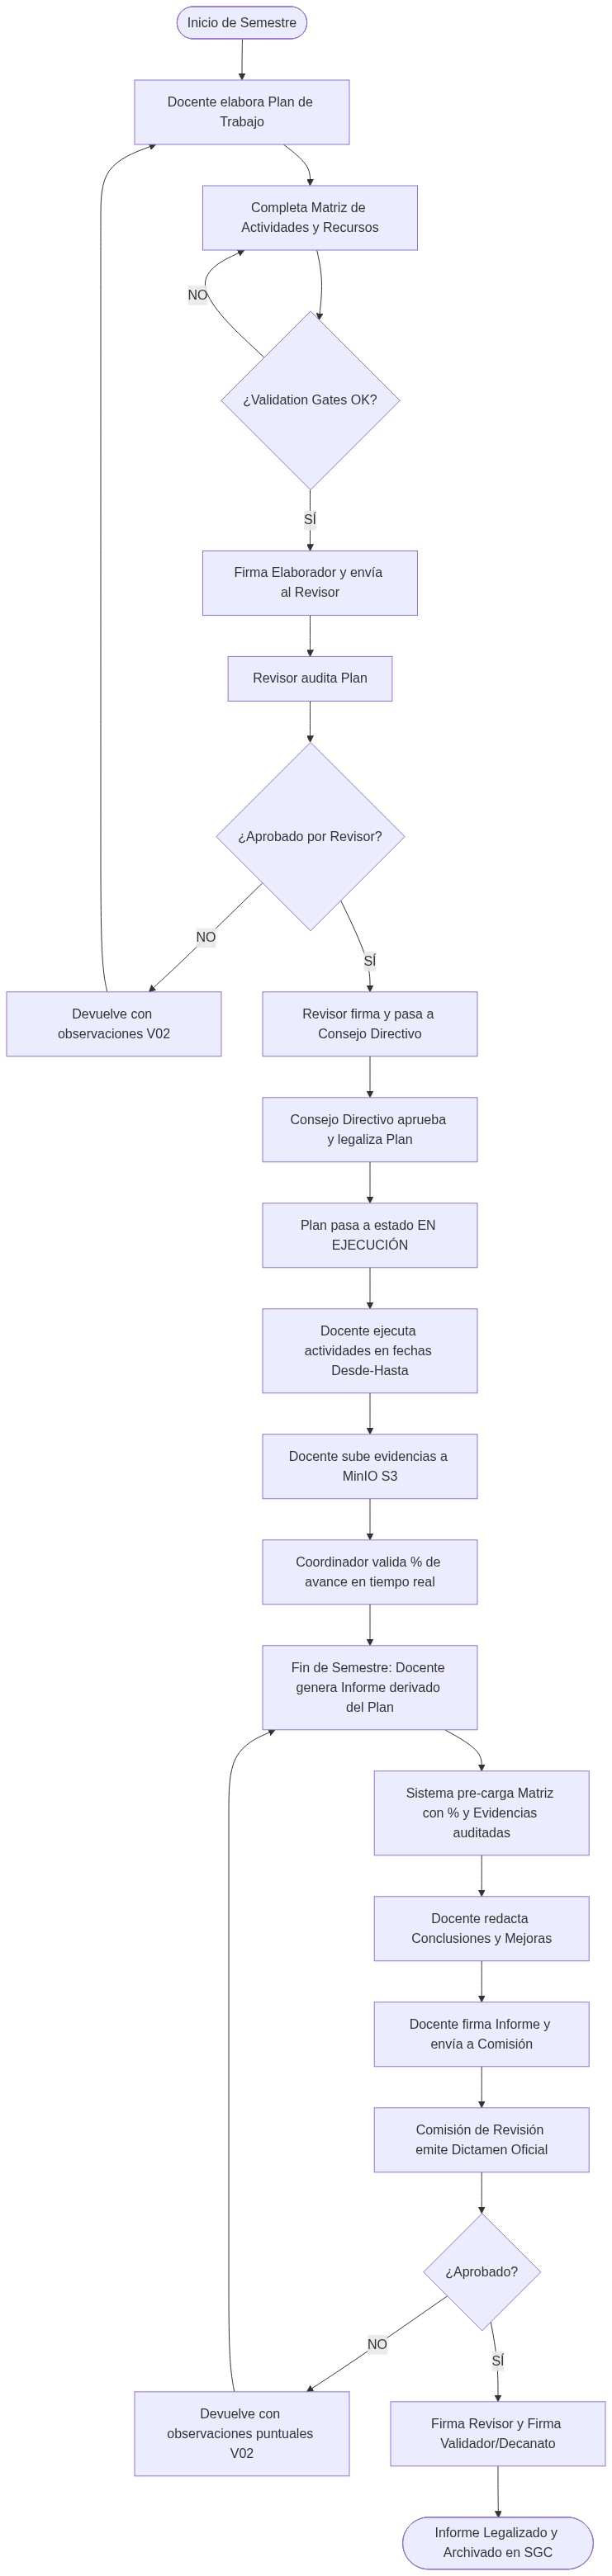
\includegraphics[width=0.88\textwidth,keepaspectratio]{images/s2_03_actividades_ciclo.png}
    \caption{Diagrama de Flujo del Proceso de Revisión por Comité y Retorno de Observaciones.}
    \label{fig:circuito_revision}
\end{figure}

\section{Descripción de actividades}

\subsection{Modelo de Datos de Observaciones (PostgreSQL 16)}
Se crearon las tablas \texttt{observaciones\_documento} y \texttt{historial\_estados}:
\begin{lstlisting}[language=SQL]
CREATE TABLE IF NOT EXISTS public.observaciones_documento (
    id SERIAL PRIMARY KEY,
    documento_id INT NOT NULL REFERENCES public.documentos(id) ON DELETE CASCADE,
    revisor_id INT NOT NULL REFERENCES public.usuarios(id),
    seccion VARCHAR(80) NOT NULL, -- 'datos', 'justificacion', 'matriz', 'evidencias'
    actividad_index INT,           -- Nro de fila observado en la matriz
    tipo_observacion VARCHAR(30) DEFAULT 'SUBSANABLE', -- 'MENOR', 'MAYOR', 'SUBSANABLE'
    contenido TEXT NOT NULL,
    estado_observacion VARCHAR(20) DEFAULT 'ABIERTA', -- 'ABIERTA', 'RESUELTA'
    created_at TIMESTAMP WITH TIME ZONE DEFAULT CURRENT_TIMESTAMP,
    resolved_at TIMESTAMP WITH TIME ZONE
);
\end{lstlisting}

\subsection{Controlador de Revisión y Dictámenes (seguimiento.controller.js)}
El endpoint \texttt{POST /api/seguimiento/:id/dictamen} valida que el usuario posea rol \texttt{COORDINADOR\_AREA} o \texttt{COORDINADOR\_CARRERA} antes de procesar el dictamen:
\begin{lstlisting}[language=JavaScript]
// Manejo de dictamen en el backend de SIGE
exports.registrarDictamen = async (req, res, next) => {
  const { id } = req.params;
  const { estado, observaciones } = req.body;
  const userId = req.user.id;
  
  if (!['APROBADO', 'OBSERVADO', 'RECHAZADO'].includes(estado)) {
    return res.status(400).json({ success: false, message: 'Estado de dictamen inválido' });
  }

  const client = await pool.connect();
  try {
    await client.query('BEGIN');
    await client.query(
      `UPDATE documentos SET estado = $1, updated_at = NOW() WHERE id = $2`,
      [estado === 'APROBADO' ? 'APROBADO_AREA' : 'OBSERVADO', id]
    );
    if (observaciones && observaciones.length > 0) {
      for (const obs of observaciones) {
        await client.query(
          `INSERT INTO observaciones_documento (documento_id, revisor_id, seccion, contenido)
           VALUES ($1, $2, $3, $4)`,
          [id, userId, obs.seccion, obs.contenido]
        );
      }
    }
    await client.query('COMMIT');
    return res.json({ success: true, message: 'Dictamen registrado exitosamente' });
  } catch (error) {
    await client.query('ROLLBACK');
    next(error);
  } finally {
    client.release();
  }
};
\end{lstlisting}

\begin{figure}[htbp]
    \centering
    
\includegraphics[width=0.88\textwidth,keepaspectratio]{images/preview_informe_cumplimiento.png}
    \caption{Bandeja de Expedientes y Vista de Auditoría para el Coordinador Académico en SIGE.}
    \label{fig:bandeja_coordinador}
\end{figure}

\section{Firmas de Responsabilidad}

\noindent
\renewcommand{\arraystretch}{1.2}
\begin{tabularx}{\textwidth}{|>{\raggedright\arraybackslash}m{2.9cm}|>{\raggedright\arraybackslash}X|>{\centering\arraybackslash}m{4.6cm}|>{\centering\arraybackslash}m{2.3cm}|}
    \hline
    \rowcolor{tableheader}
    \textbf{ACCIÓN} & \textbf{NOMBRE Y CARGO} & \textbf{FIRMA} & \textbf{FECHA} \\
    \hline
    \textbf{Elaborado por:} & Heidi Villavicencio\newline Analista de Requisitos / UI-UX & \parbox[c]{4.4cm}{\centering\vspace{4pt}
\includegraphics[height=1.5cm,width=4.0cm,keepaspectratio]{images/firma_heidi.png}\vspace{4pt}} & 02/10/2026 \\
    \hline
    \textbf{Revisado por:} & Steeven Toala\newline Líder de Proyecto / Arquitecto & \parbox[c]{4.4cm}{\centering\vspace{4pt}
\includegraphics[height=1.5cm,width=4.0cm,keepaspectratio]{images/firma_steveen.png}\vspace{4pt}} & 02/10/2026 \\
    \hline
    \textbf{Revisado por:} & Nixon Hurtado\newline Desarrollador Backend / DBA & \parbox[c]{4.4cm}{\centering\vspace{8pt}\textbf{[ FIRMADO ELECTRÓNICAMENTE ]}\vspace{8pt}} & 02/10/2026 \\
    \hline
    \textbf{Revisado por:} & Andrea Vásquez\newline Desarrolladora Frontend / QA & \parbox[c]{4.4cm}{\centering\vspace{8pt}\textbf{[ FIRMADO ELECTRÓNICAMENTE ]}\vspace{8pt}} & 02/10/2026 \\
    \hline
    \textbf{Aprobado por:} & Ing. Paulo Torres, Mg.\newline Docente Evaluador -- Gestión Proyectos & \parbox[c]{4.4cm}{\centering\vspace{8pt}\textbf{\textcolor{gray!80}{\scriptsize [ PENDIENTE DE APROBACIÓN ]}}\vspace{8pt}} & \textbf{\textcolor{gray!90}{Pendiente}} \\
    \hline
\end{tabularx}

\vspace{0.4cm}

\section{Control de Cambios}

\noindent
\renewcommand{\arraystretch}{1.2}
\begin{tabularx}{\textwidth}{|>{\hsize=0.45\hsize\centering\arraybackslash}X|>{\hsize=1.55\hsize\raggedright\arraybackslash}X|>{\hsize=1.2\hsize\raggedright\arraybackslash}X|>{\hsize=0.8\hsize\centering\arraybackslash}X|}
    \hline
    \rowcolor{tableheader}
    \textbf{Versión} & \textbf{Descripción del cambio} & \textbf{Responsable del cambio} & \textbf{Fecha de aprobación} \\
    \hline
    1.0 & Creación e implementación formal del módulo de revisión académica, bitácora de observaciones y máquina de estados. & Steeven Toala / Nixon Hurtado & 02/10/2026 \\
    \hline
\end{tabularx}

\vspace{0.4cm}

\section{Anexos}

\subsection*{Anexo 1: Tabla de Transición de Estados del Expediente Académico}
\begin{table}[H]
\centering
\small
\begin{tabularx}{\textwidth}{|l|l|X|}
\hline
\rowcolor{tableheader}
\textbf{Estado Inicial} & \textbf{Acción Disparadora} & \textbf{Estado Destino y Permisos} \\ \hline
\texttt{BORRADOR} & Enviar a Revisión (Docente) & \texttt{ENVIADO\_REVISION} (Bloqueo de edición para docente) \\ \hline
\texttt{ENVIADO\_REVISION} & Emitir Observaciones (Comité) & \texttt{OBSERVADO} (Edición habilitada exclusivamente en secciones observadas) \\ \hline
\texttt{OBSERVADO} & Subsanar y Reenviar (Docente) & \texttt{SUBSANADO} (Re-ingreso a bandeja de revisión) \\ \hline
\texttt{ENVIADO\_REVISION} & Dictamen Favorable (Comité) & \texttt{APROBADO\_AREA} (Habilita el siguiente nivel de firma) \\ \hline
\end{tabularx}
\caption{Matriz de Transición de Estados Documentales en SIGE.}
\label{tab:estados_transicion}
\end{table}

\end{document}
